% 1958 年北京卷第 11 题：⊙O、过 A、B 两点的切线及其交点、与弧 AB 和两切线相切的圆 ⊙M（按源卷布局；切线交点 C 原卷图中未标注字母，故不标）
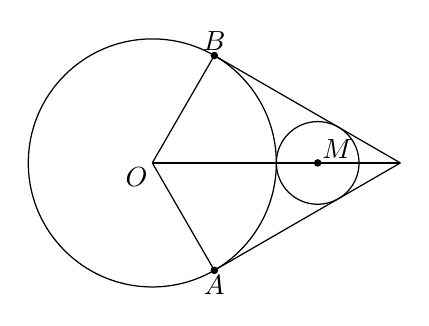
\begin{tikzpicture}[scale=1.05, line width=0.45pt,
  every node/.style={inner sep=1.5pt}]
  \coordinate (O) at (0,0);
  \coordinate (B) at (0.75,1.299);
  \coordinate (A) at (0.75,-1.299);
  \coordinate (M) at (2,0);
  \coordinate (C) at (3,0);
  \draw (O) circle (1.5);
  \draw (M) circle (0.5);
  \draw (O) -- (C);
  \draw (O) -- (B);
  \draw (O) -- (A);
  \draw (B) -- (C);
  \draw (A) -- (C);
  \fill (A) circle (1.3pt);
  \fill (B) circle (1.3pt);
  \fill (M) circle (1.3pt);
  \node[anchor=north east] at (O) {$O$};
  \node[anchor=south] at (B) {$B$};
  \node[anchor=north] at (A) {$A$};
  \node[anchor=south west] at (M) {$M$};
\end{tikzpicture}
